\section {Results of the $\nueb$ Appearance Analysis}
\label{sec:results}
The rate-only and rate+shape p-values for $\nueb$ appearance are performed on the combined \RunPeriod statistics following the same procedure as in Sec \ref{sec:method}. 1-sided p-values are computed on the right tail of the test statistic expected distribution to exclude $\beta = 0$ and the left tail to exclude $\beta = 1$. Fig \ref{fig:asimova_spectra_all} shows the data in the 5 Super-K event samples overlaid with the expected event rates for Asimov data set A. A summary of the observed number of events in Super-K, $\Delta \chi^2$ and p-values is given in Tab \ref{tab:data_comparison_R19c_R17}.



In Figs \ref{fig:data_rate-only} and \ref{fig:data_rate+shape} the distributions of the test statistic, for rate-only and rate+shape analyses, are shown and compared with the data. Tab \ref{tab:data_comparison_R19c_R17} contains a summary of the results. The rate-only analysis disfavours each hypothesis almost equally, whilst the rate+shape analysis disfavours the $\beta = 1$ hypothesis more than the $\beta = 0$ hypothesis. The Jeffreys scale indicates that the Bayes factor of \BayesFactorData\ corresponds to a poor preference for the $\beta = 0$ hypothesis over $\beta = 1$. %In comparison to the Run 1-7 analyses, the preference for $\beta = 0$ remains but has grown weaker. 
In comparison to the Run 1-7 analysis, the rate-only $\beta = 0$ p-value has decreased by a factor of 0.51. This is due to the number of observed events per POT increasing by a factor of 1.5, increasing the amount that the $\beta = 0$ hypothesis is disfavoured. The rate+shape $\beta = 0$ p-value has decreased by a factor of 0.57. In addition to the number of observed events per POT increasing by a factor of 1.5, this can be explained by an increase in the number of events (compared to the Run 1-7 analysis \cite{OurRun16AntiNueBarAppearanceAnalysis3Flavour}) in regions of the spectra in Fig \ref{fig:nuebar_tot_spectra} where a larger number of events are expected.

The P-theta rate-only p-values for the \RunPeriod data set are \PthetaPvalDataRateOnlyBetaZero\ and \PthetaPvalDataRateOnlyBetaOne\ for $\beta = 0$ and $\beta = 1$, respectively and the rate+shape p-values (using $E_{reco}-\theta$) are \PthetaPvalDataRateShapeErecThetaBetaZero\ and \PthetaPvalDataRateShapeErecThetaBetaOne\ for $\beta = 0$ and $\beta = 1$, respectively \cite{PthetaR19cNuebarAppearance}. The p-values produced by the VALOR and P-theta groups are considered to be within acceptable agreement. {\color{red} During the Run1-9c analysis,} the reason for the remaining differences between the VALOR and P-theta p-values {\color{red}were} thought to be due to differences in the toy generation methods. {\color{red} A comparison of the toy generation methods is shown in appendix \ref{app:sampling_vs_reweighting} using full Run 1-9 statistics.}

By breaking the electron-like antineutrino mode spectra from Fig \ref{fig:asimova_spectra_all} into its components, as shown in Fig \ref{fig:asimova_spectra_components}, some explanation can be offered for the preference for the no $\nueb$ appearance hypothesis. The observed events do not appear to fit the Asimov A expected $\numub \rightarrow \nueb$ distribution well, instead they are more consistent with the $\numu \rightarrow \nue$ and intrinsic $\nue\ \&\ \nueb$ backgrounds. As the shape of the spectra discredits the $\beta = 1$ hypothesis (which is information that the rate-only analysis does not have access to), the $\beta = 1$ p-value for the rate+shape analysis is substantially smaller than that of the rate-only analysis.

\FloatBarrier

\begin{figure*}[htb]
	\center
	\begin{subfigure}[b]{0.49\textwidth}
		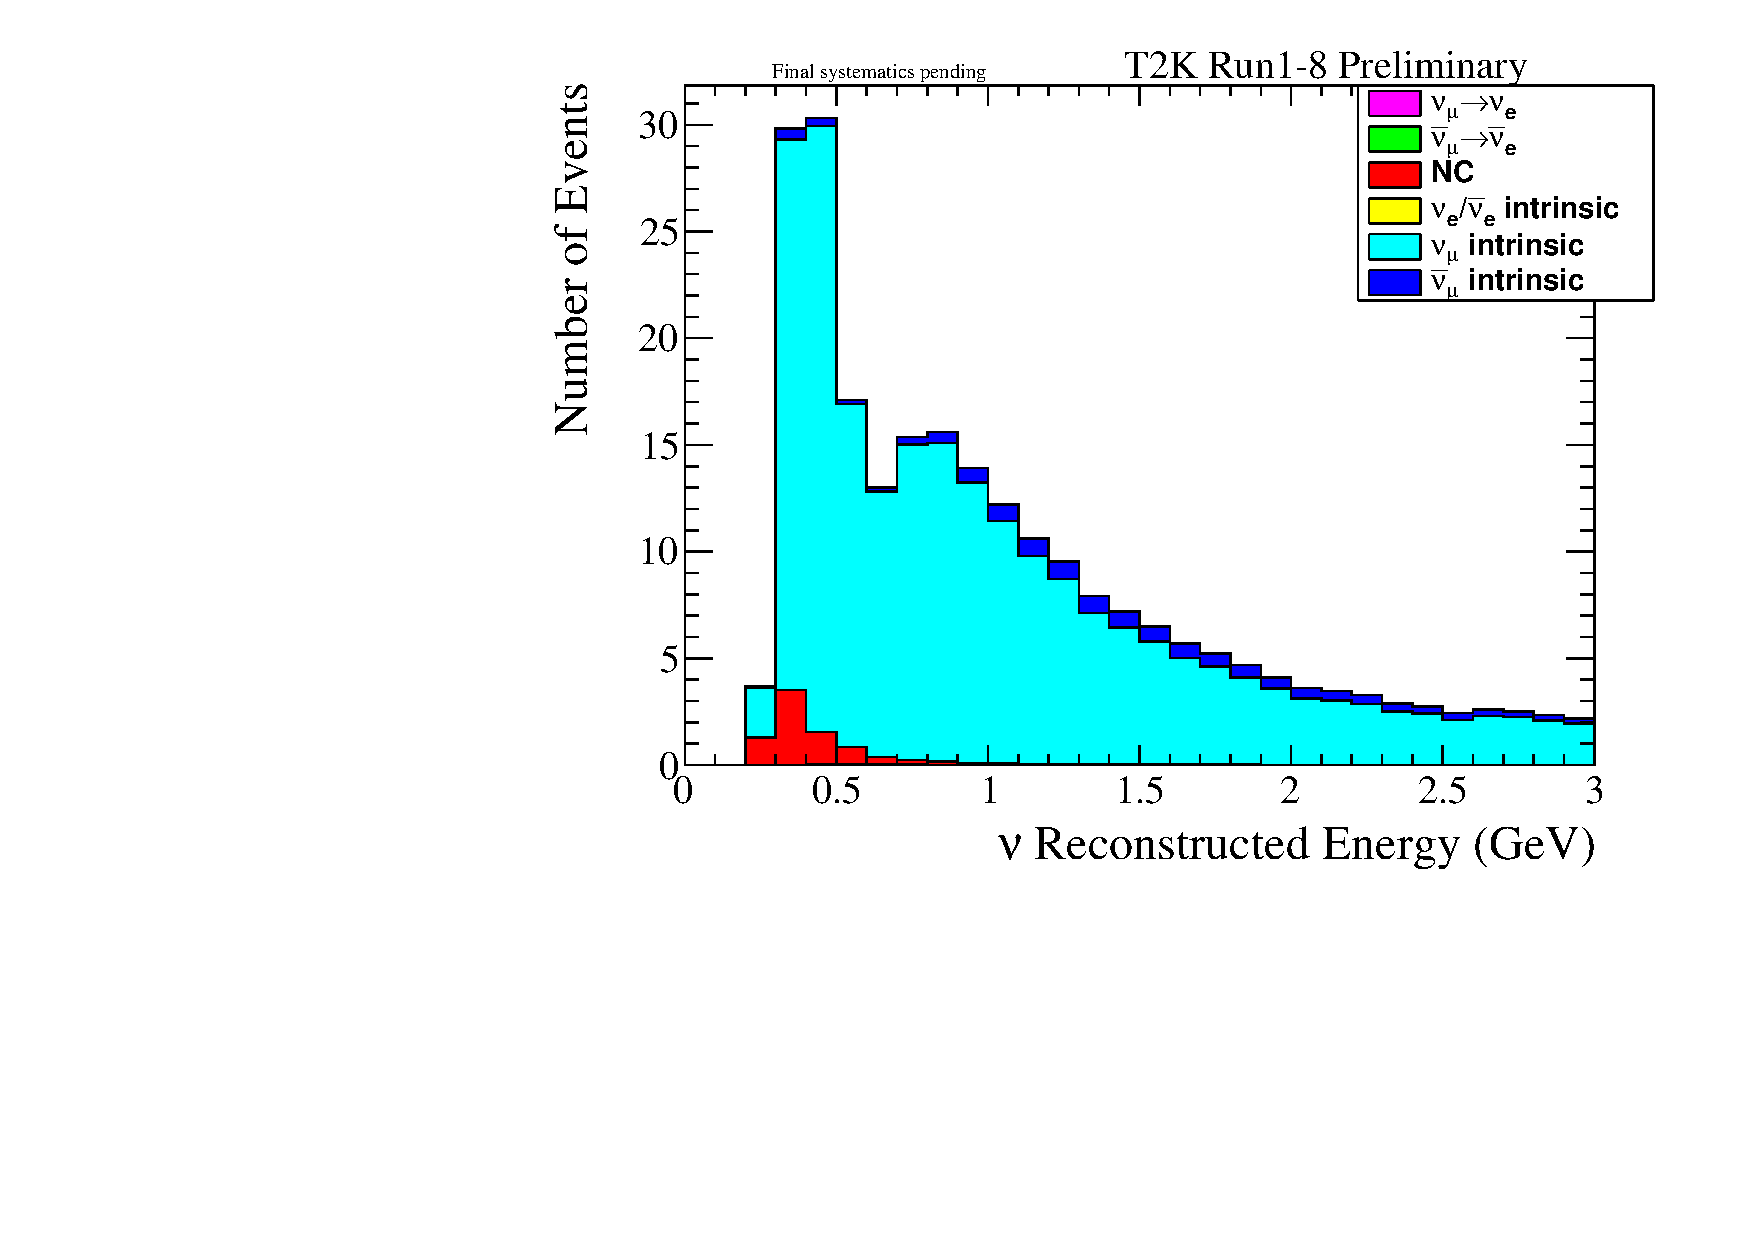
\includegraphics[width=0.9\textwidth]{spectra/spectrum_osc_asimova_1Rmu}
		\caption{Muon-like, neutrino mode}
	\end{subfigure}
	\begin{subfigure}[b]{0.49\textwidth}
		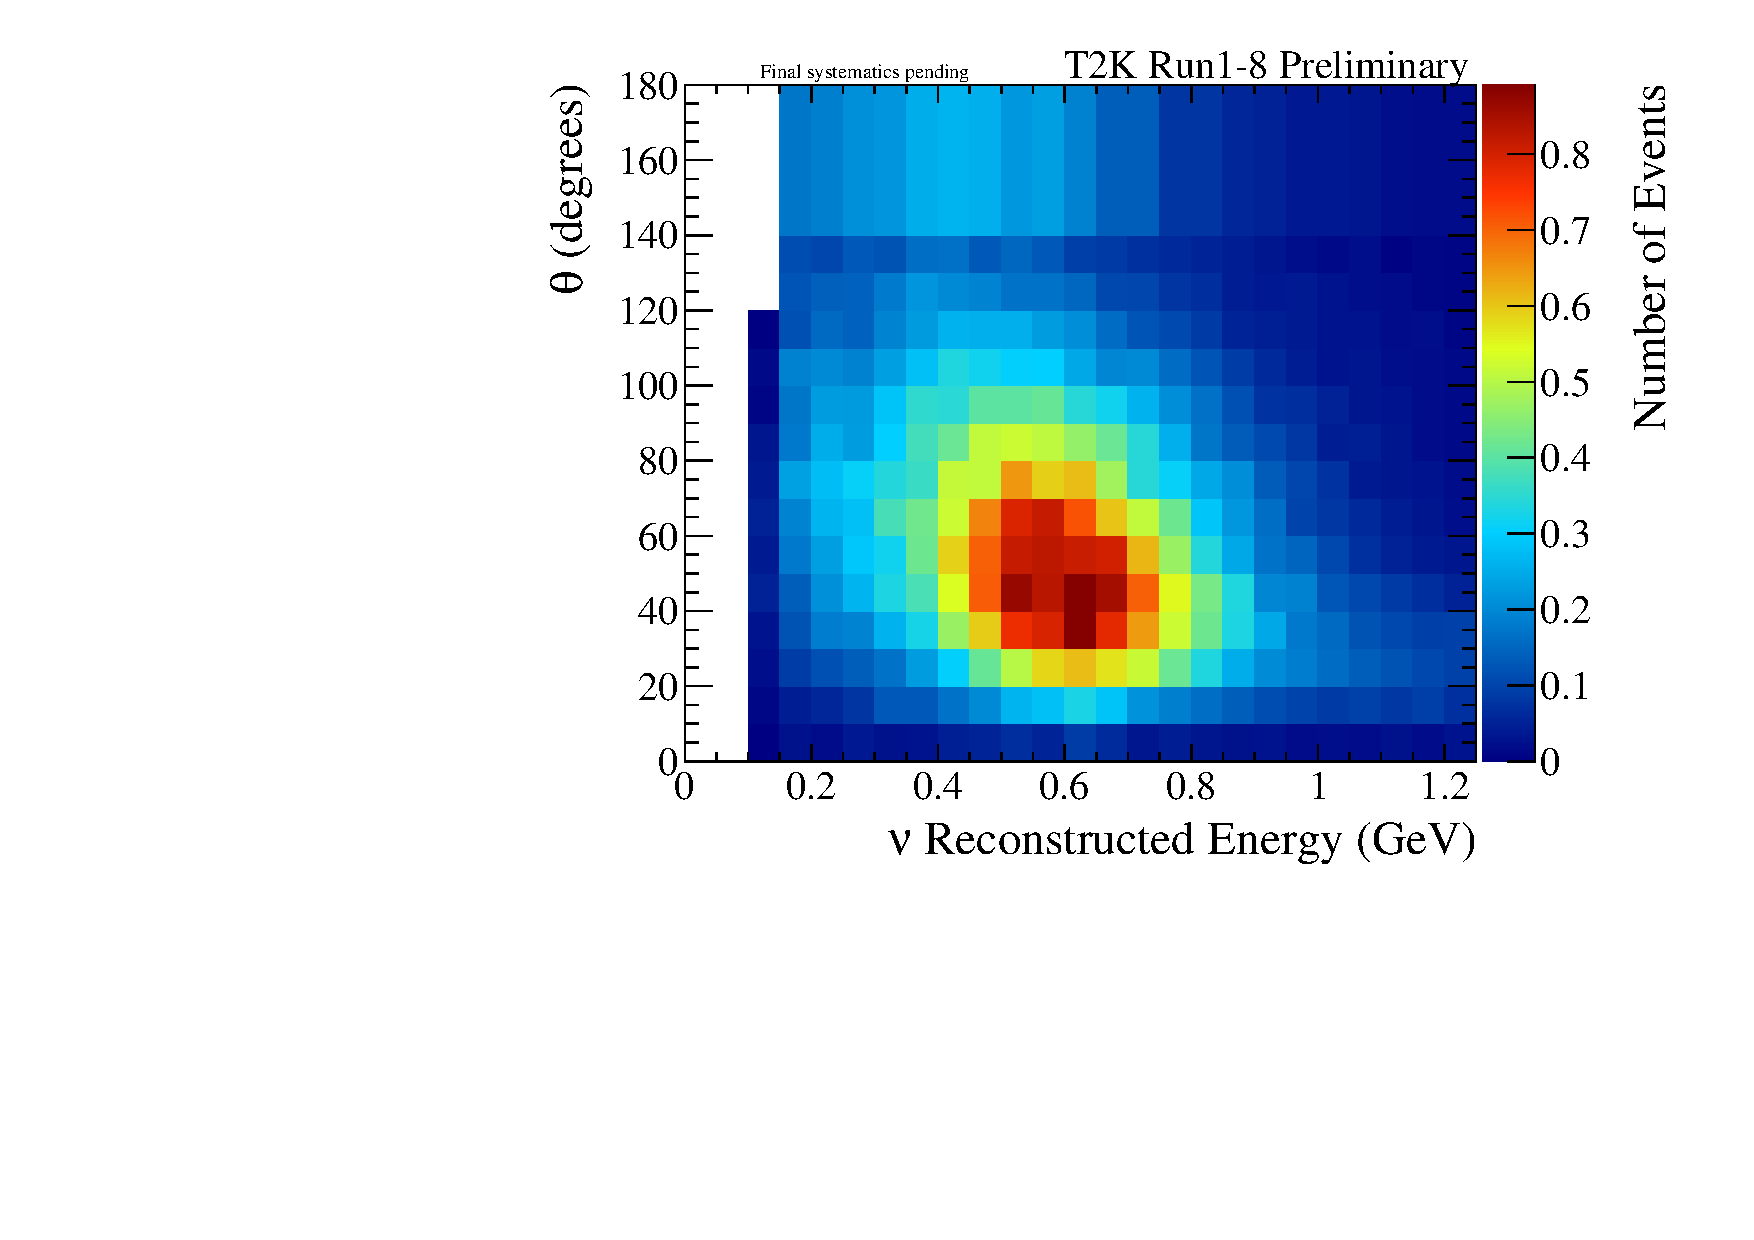
\includegraphics[width=0.9\textwidth]{spectra/spectrum_osc_asimova_1Re}
		\caption{Electron-like, neutrino mode}
	\end{subfigure}
	\begin{subfigure}[b]{0.49\textwidth}
		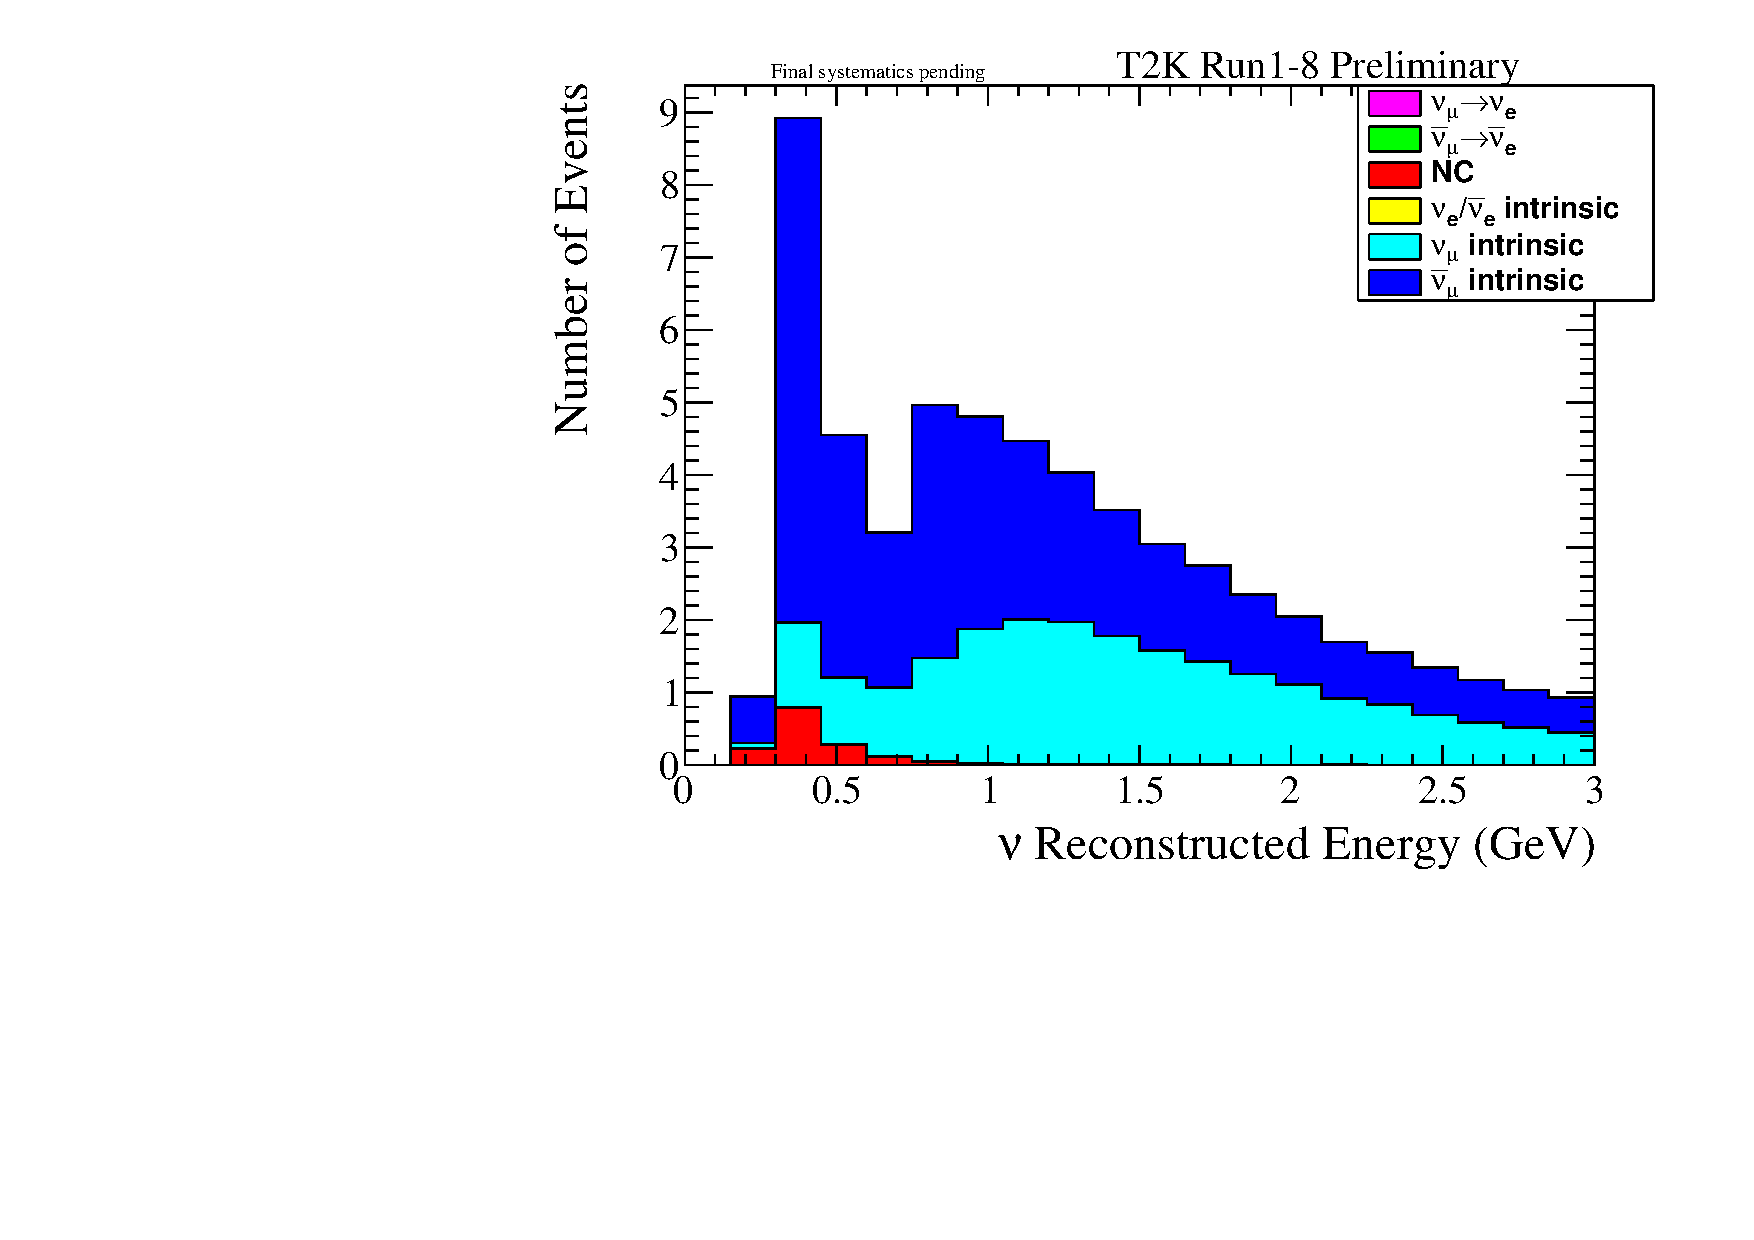
\includegraphics[width=0.9\textwidth]{spectra/spectrum_osc_asimova_RHC1Rmu}
		\caption{Muon-like, antineutrino mode}
	\end{subfigure}
	\begin{subfigure}[b]{0.49\textwidth}
		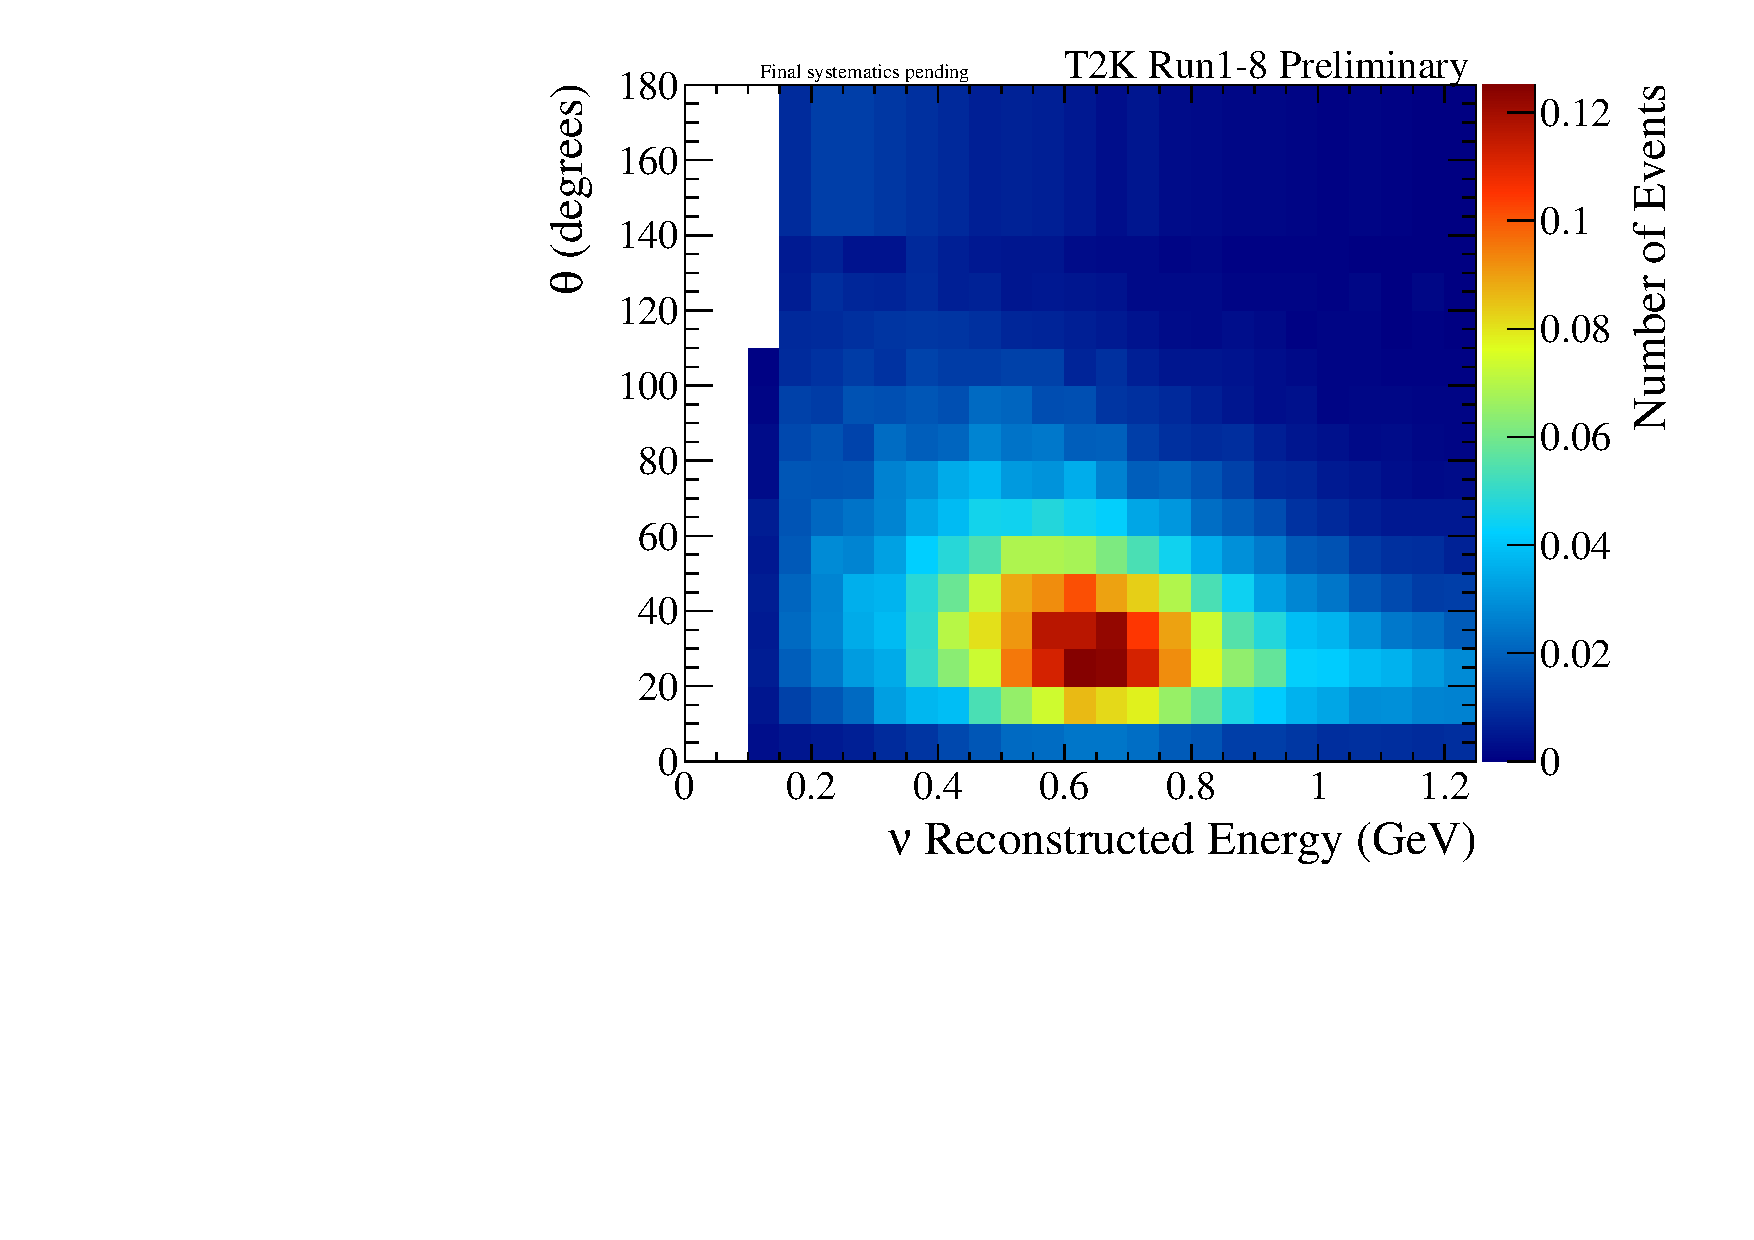
\includegraphics[width=0.9\textwidth]{spectra/spectrum_osc_asimova_RHC1Re}
		\caption{Electron-like antineutrino mode}
	\end{subfigure}
	\begin{subfigure}[b]{0.49\textwidth}
		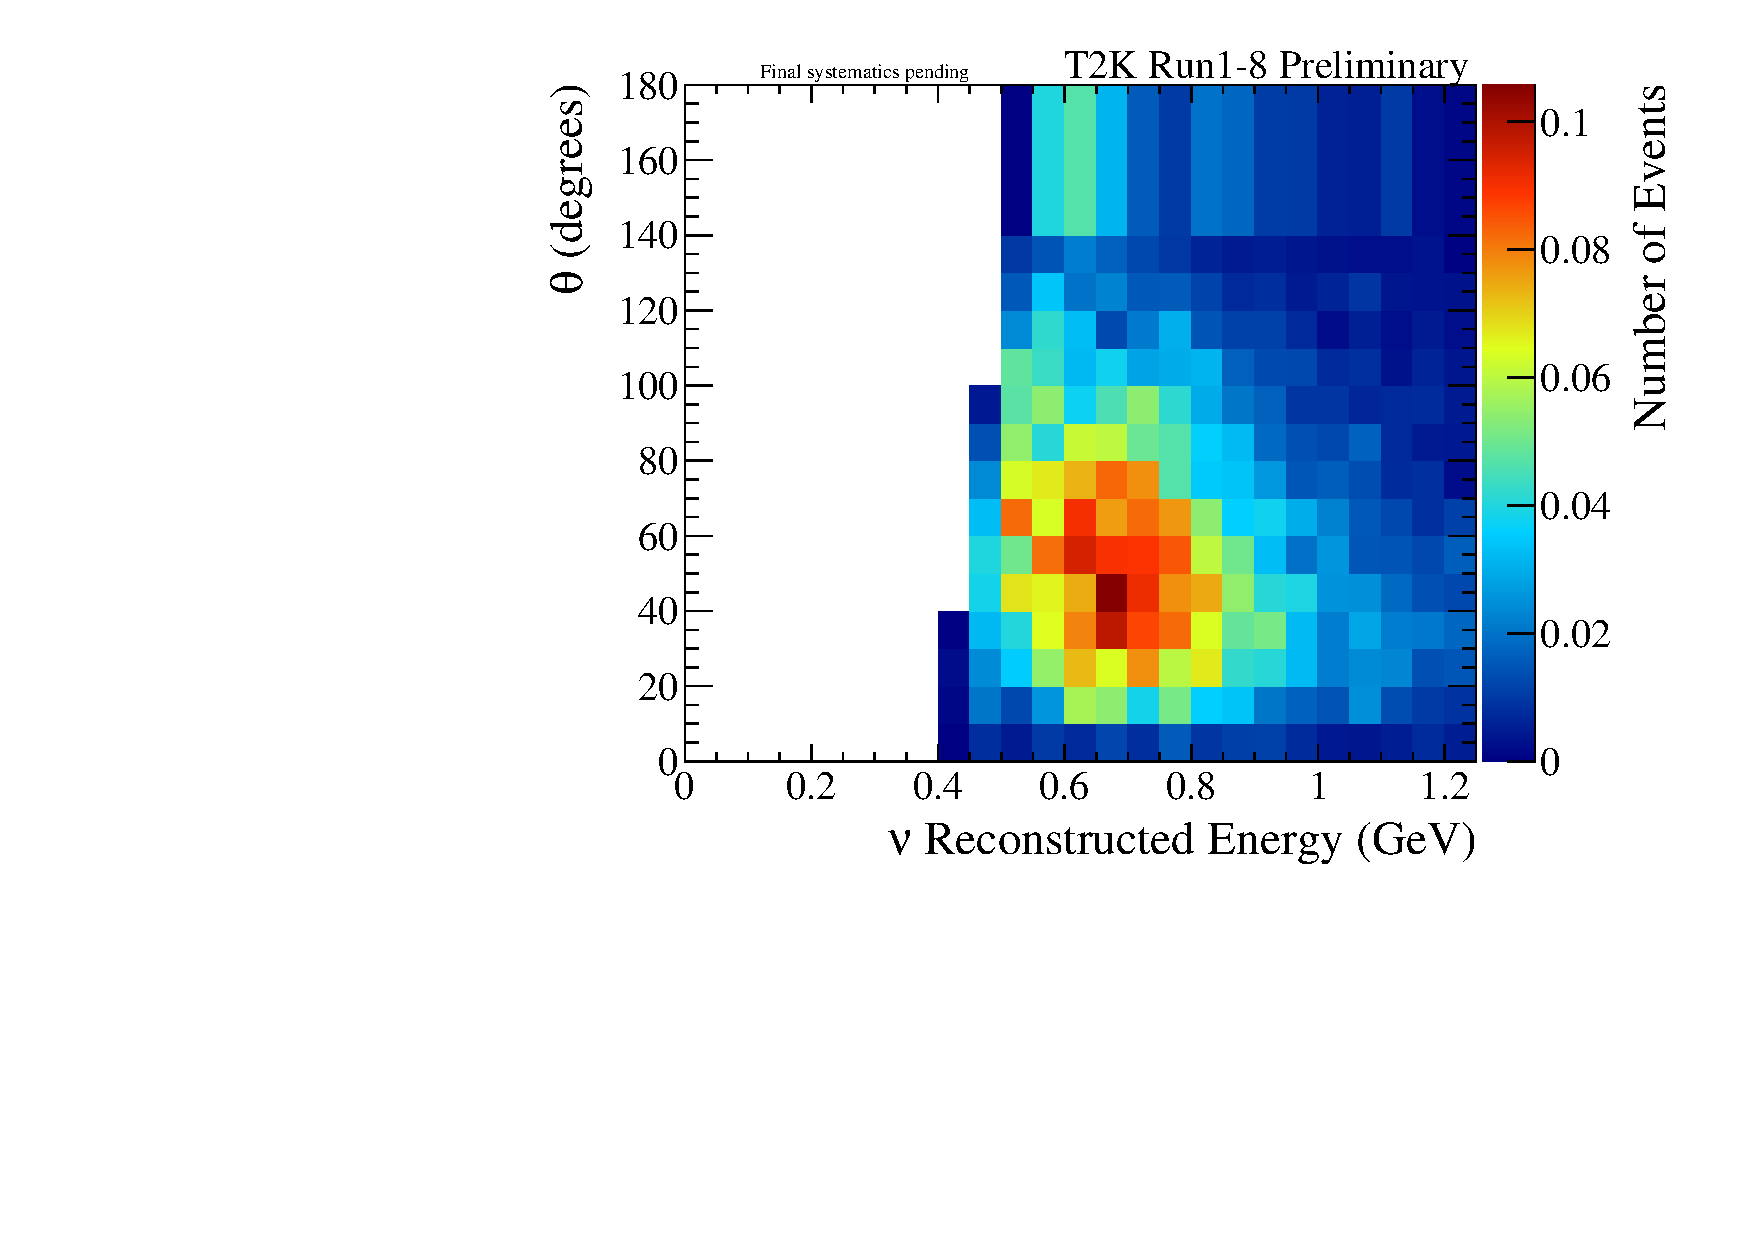
\includegraphics[width=0.9\textwidth]{spectra/spectrum_osc_asimova_MultiRe}
		\caption{\nueCConepi-like, neutrino mode}
	\end{subfigure}
	\caption {
		Predicted Asimov A spectra. $\mu$-like distributions are a function of the reconstructed neutrino energy, while the $e$-like, including \nueCConepi, distributions are functions of both the reconstructed neutrino energy and the reconstructed angle between the outgoing lepton and the neutrino direction. The distributions correspond to the statistics collected in the full \RunPeriod data set. The spectra are generated with the systematic parameters described in \cref{sec:systematics} and the oscillation parameters corresponding to the Asimov data set A shown in \cref{tab:asimov_definition1}.
	}
	\label{fig:asimova_spectra_all}
\end{figure*}
\clearpage

\begin{figure}
	\centering
	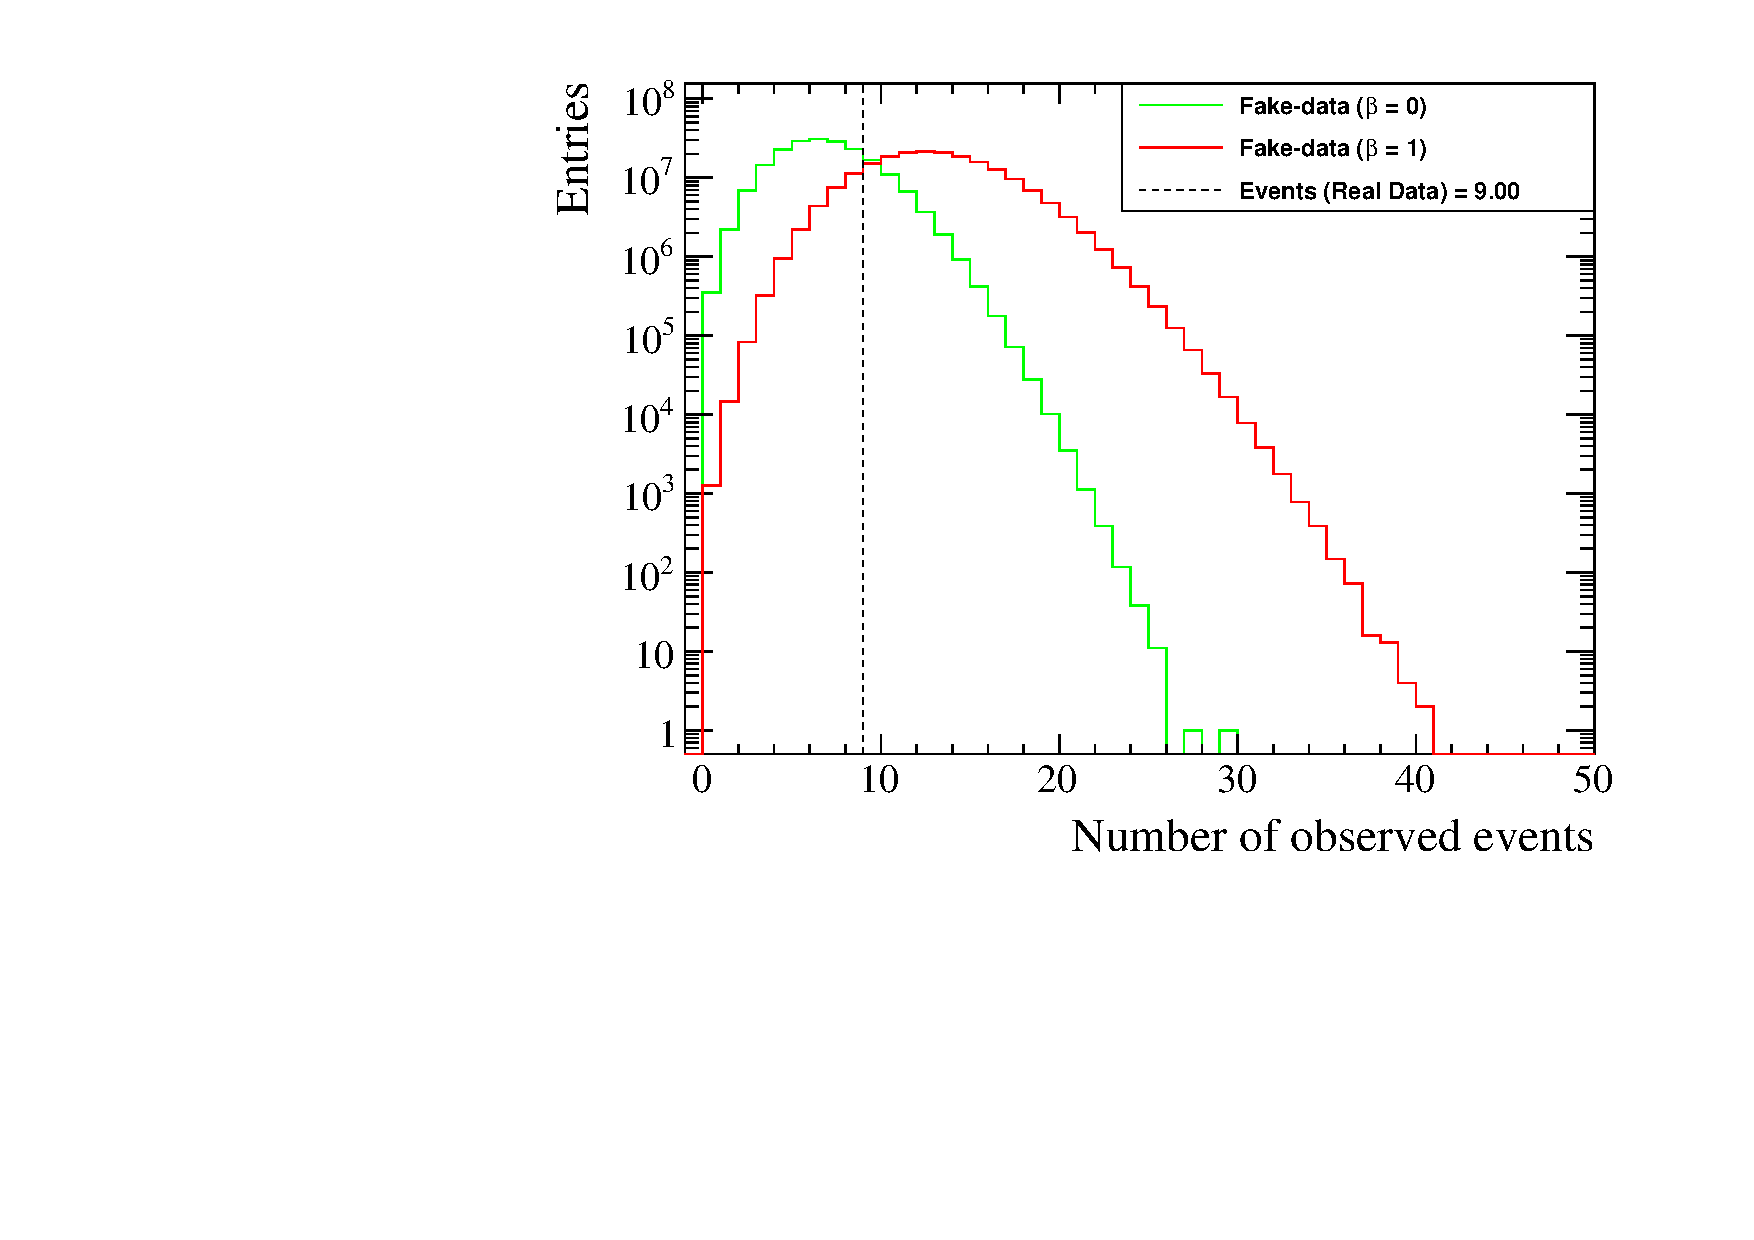
\includegraphics[scale=0.65]{data/nuebarapp_graphs_nmargtoys=200k_nexp=20k_rate-only_posterior-predictive_VALORonly_nevents}
	\caption{The distribution of the total number of events in the antineutrino mode single-ring e-like sample from each of the \NToysFakeDataRateOnly\ toy experiments for both the $\beta = 0$ and $\beta = 1$ hypotheses. The distributions were produced using the method outlined in section \ref{sec:method_rate-only} using the \RunPeriod data spectra to calculate the 4-sample likelihood. The dashed line corresponds to the total number of events given by the \RunPeriod data set.
	}
	\label{fig:data_rate-only}
\end{figure}

\begin{figure}
	\centering
	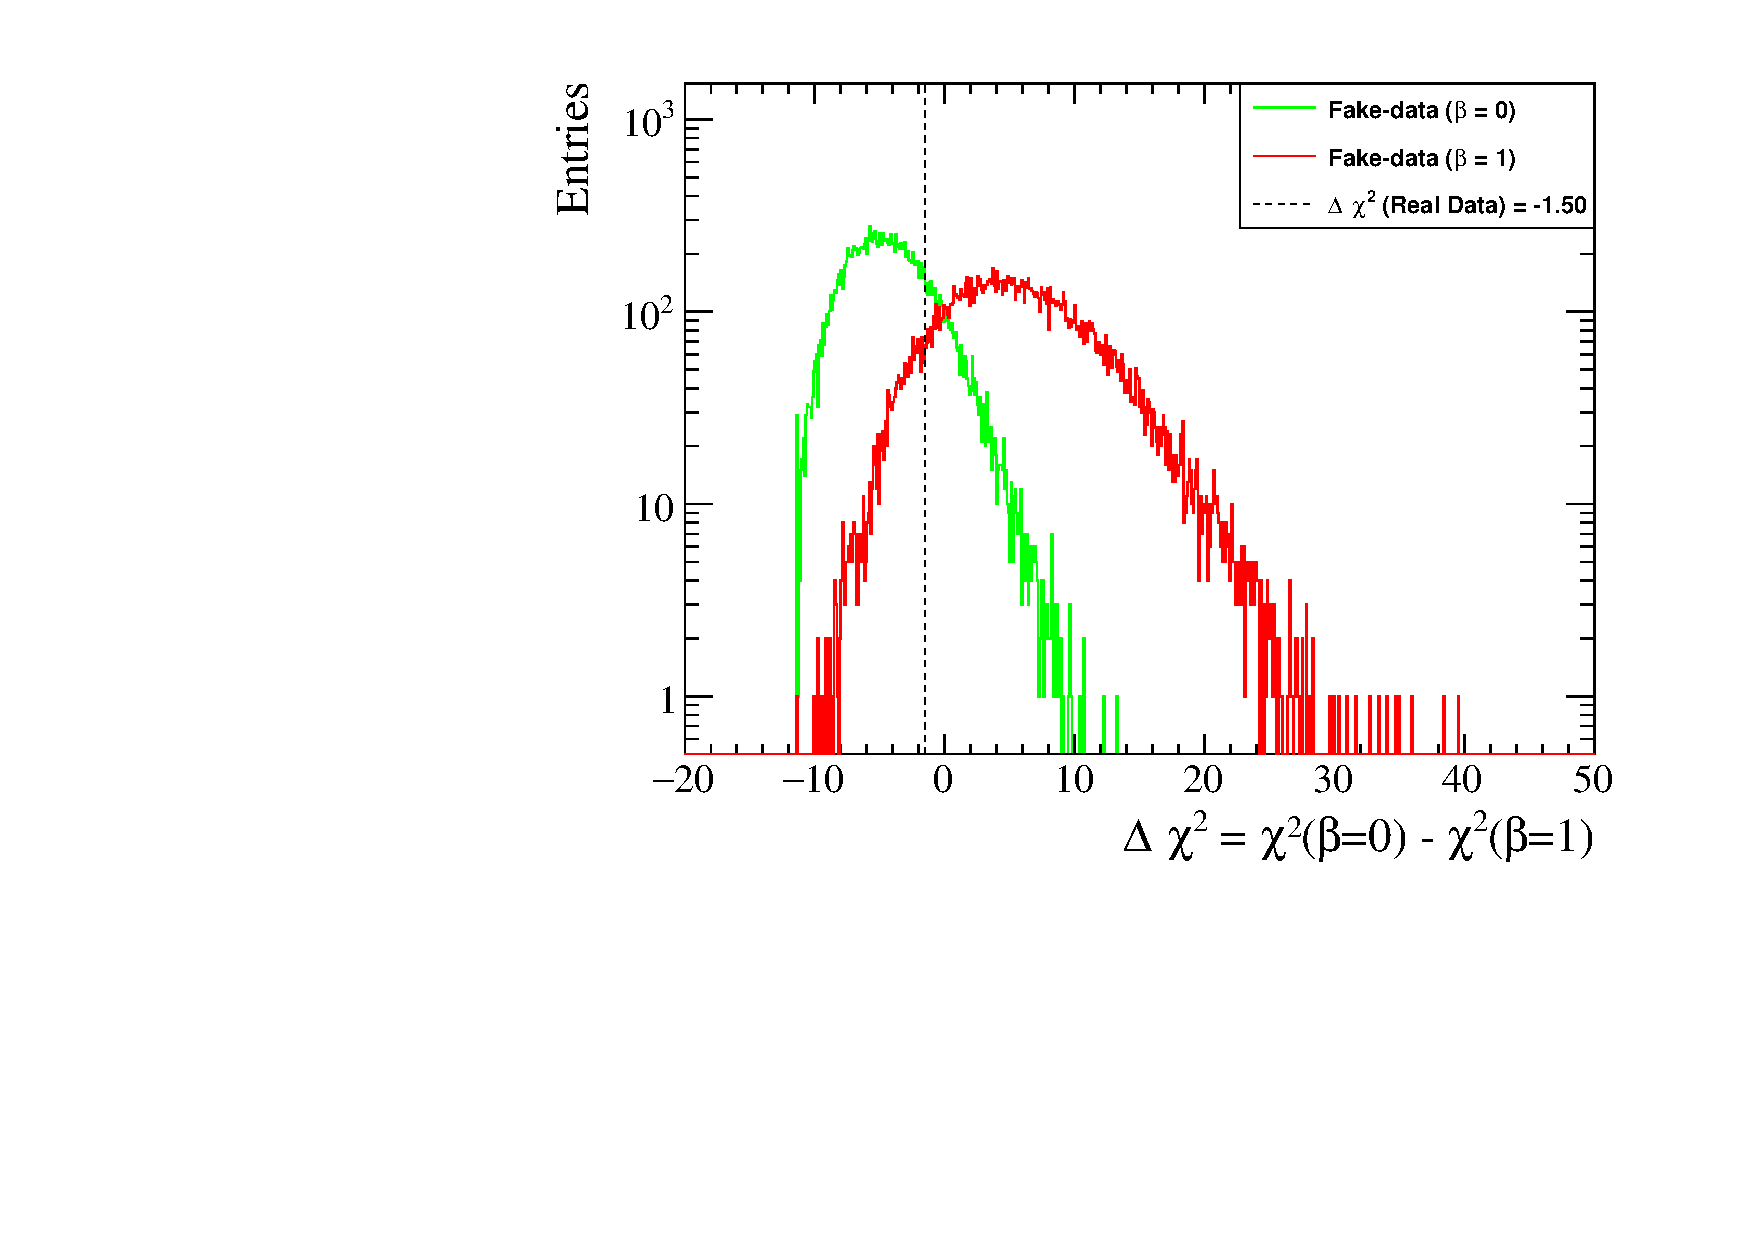
\includegraphics[scale=0.65]{data/nuebarapp_graphs_nmargtoys=200k_nexp=20k_rate+shape_posterior-predictive_VALORonly_Deltachisq_logscale}
	\caption{The distribution of $\Delta \chi^2$ values from each of the \NToysFakeDataRatePlusShape\ toy experiments for both the $\beta = 0$ and $\beta = 1$ hypotheses. The distributions were produced using the method outlined in section \ref{sec:method_rate+shape} using the \RunPeriod data spectra to calculate the 4-sample likelihood. The dashed line corresponds to the $\Delta \chi^2$ value given by the \RunPeriod data set.
	}
	\label{fig:data_rate+shape}
\end{figure}

\FloatBarrier

\begin{table}
	\centering
	\begin{tabular}{|c|c|c|c|c|c|c|c|c|}
		\hline
		\multirow{2}{*}{Run} & \multirow{2}{*}{RHC POT}   & \multicolumn{3}{|c|}{Rate-only Analysis}  			    & \multicolumn{4}{|c|}{Rate+shape Analysis} \\
		\cline{3-9}     				
		     		&                            & $N_{obs}$  					& $\beta = 0$ p-value       & $\beta = 1$ p-value      & $\Delta \chi^2_{\textrm{obs}}$  & $\beta = 0$ p-value        & $\beta = 1$ p-value       & \textbf{$B_{01}$} \\
		\hline
		1-9c  & \TotalPotNuBarRunOneNineC  & \NskObservedNueBarRunOneNineC & \pvalRateOnlyBetaZeroData & \pvalRateOnlyBetaOneData & \DeltachisqData  & \pvalRateShapeBetaZeroData & \pvalRateShapeBetaOneData & \BayesFactorData \\
		\hline
		1-7     & \TotalPotNuBarRunOneSevenC & 4			  					& 0.410						& 0.2155				   & -1.930			  & 0.3742					   & 0.099					  & 2.62 \\
		\hline
	\end{tabular}
	\caption{Summary of observed number of events, $\Delta \chi^2$, rate-only and rate+shape p-values and Bayes factor from the combined \RunPeriod data set compared to the Run 1-7 data set used for the previous iteration of this analysis, in 2016 \cite{OurRun16AntiNueBarAppearanceAnalysis3Flavour}.}
	\label{tab:data_comparison_R19c_R17}
\end{table}

%TODO: POT column as well?


\begin{figure*}[htb]
	\center
	\begin{subfigure}[b]{0.49\textwidth}
		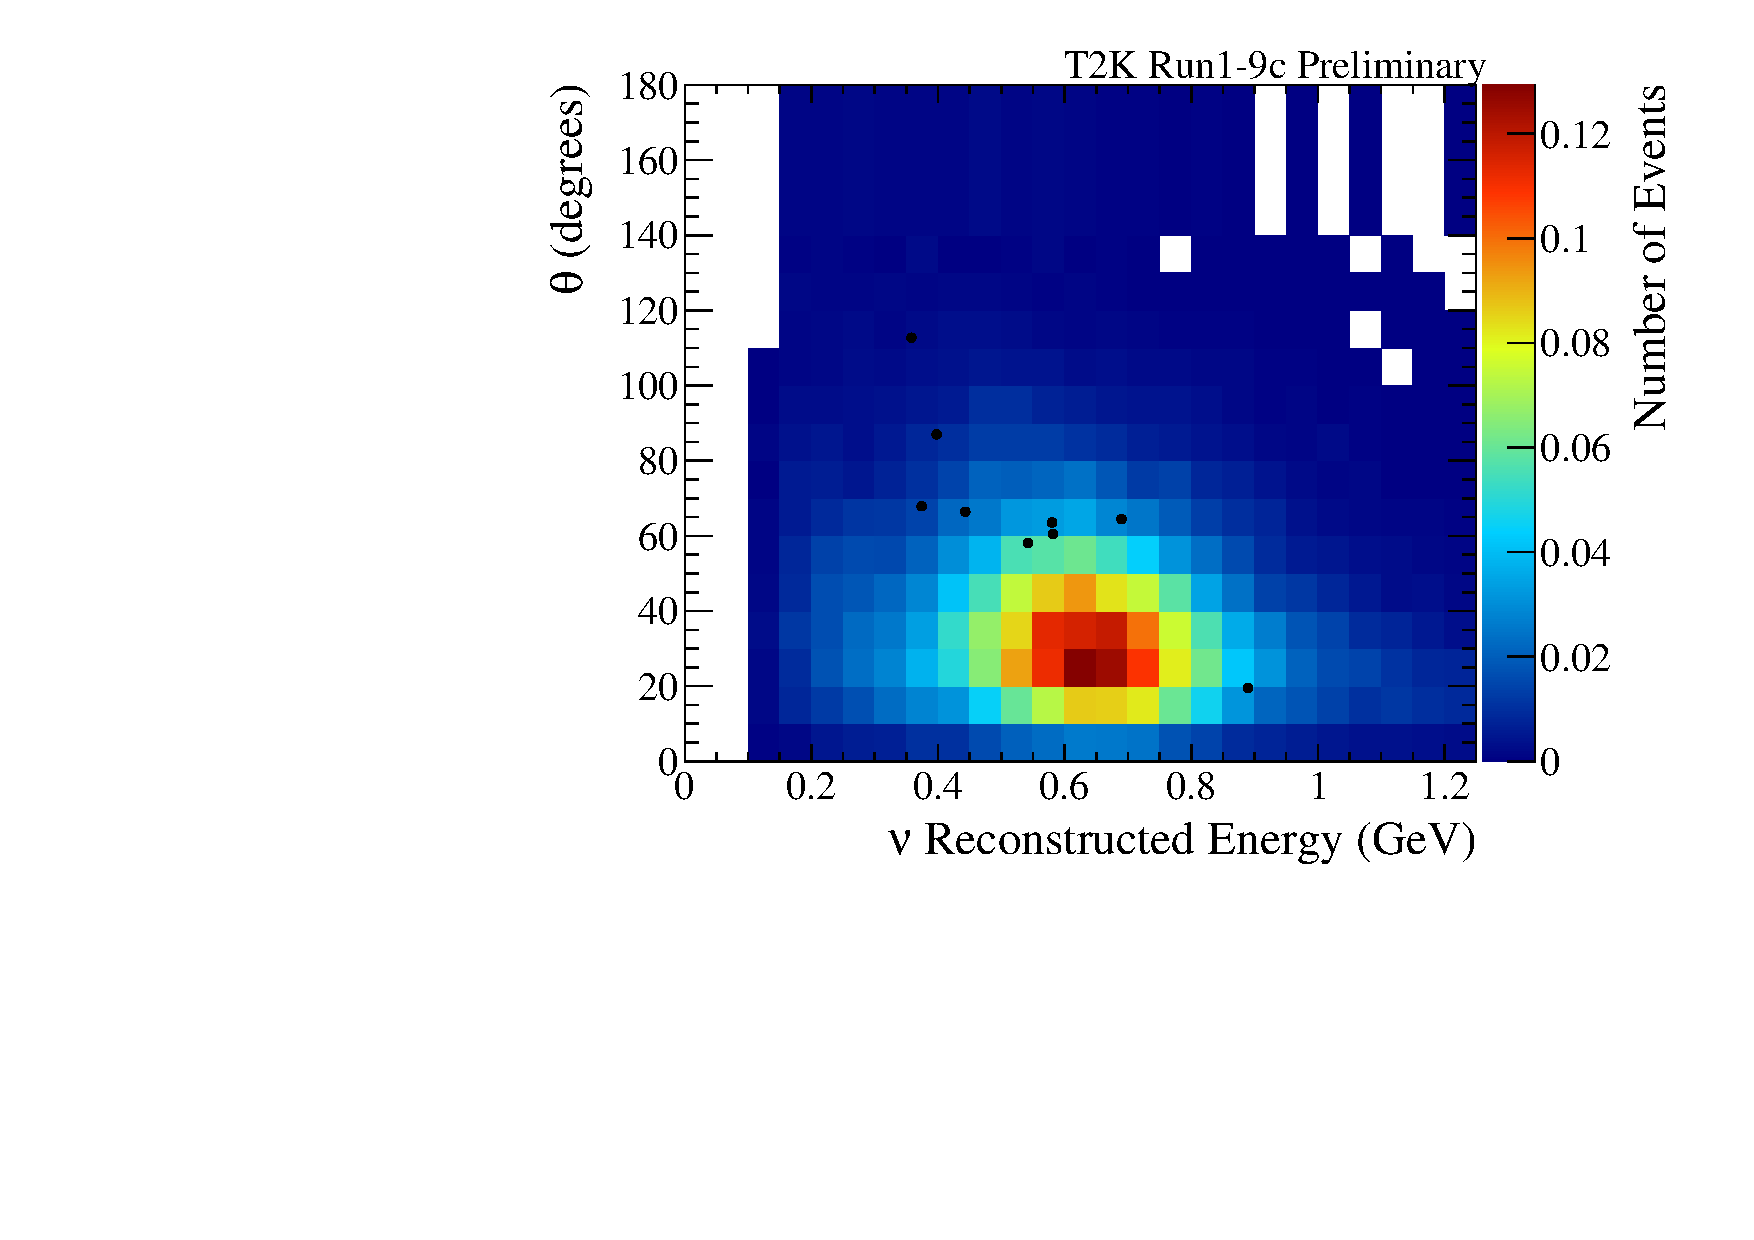
\includegraphics[width=0.9\textwidth]{spectra/components/spectrum_AsmovA_RHC1Re_NumuBarToNueBar}
		\caption{$\numub \rightarrow \nueb$}
	\end{subfigure}
	\begin{subfigure}[b]{0.49\textwidth}
		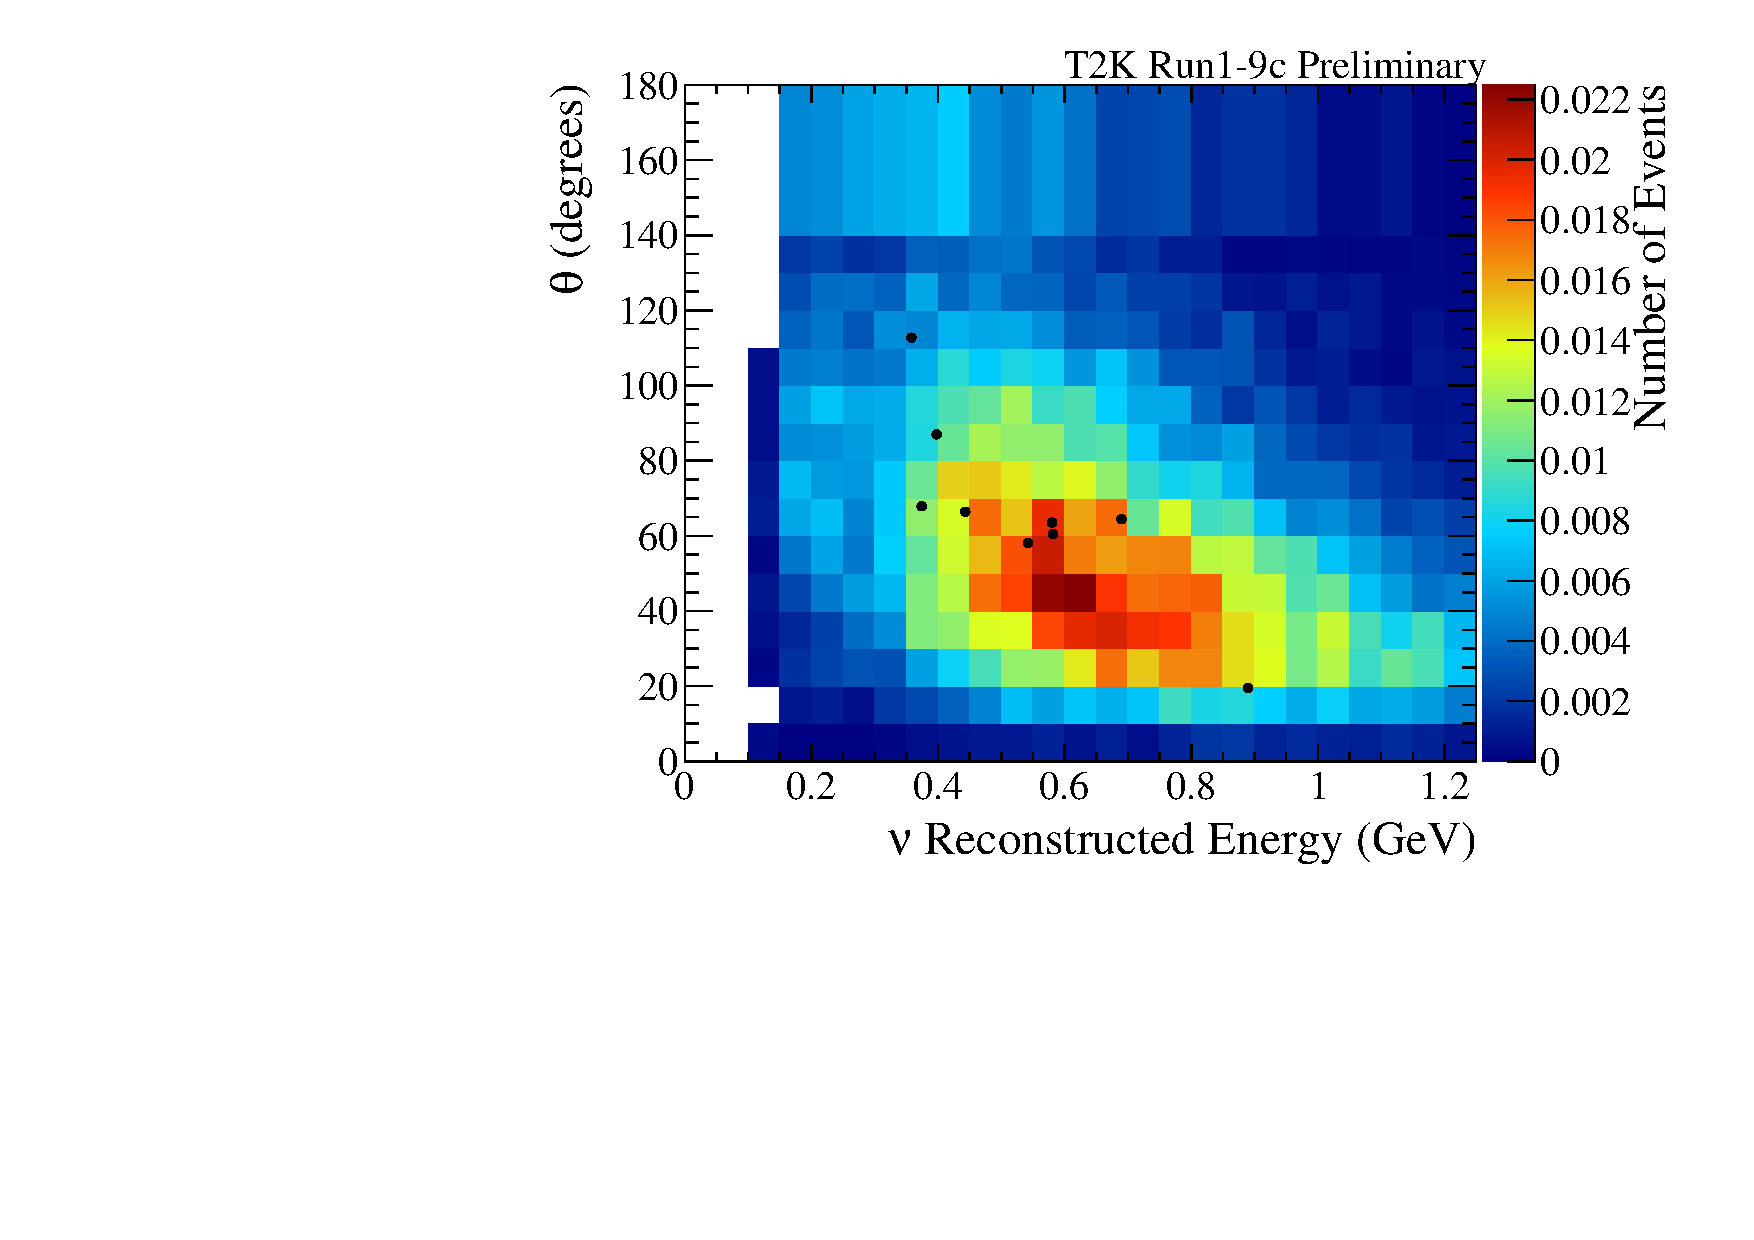
\includegraphics[width=0.9\textwidth]{spectra/components/spectrum_AsmovA_RHC1Re_NumuToNue}
		\caption{$\numu \rightarrow \nue$}
	\end{subfigure}
	\begin{subfigure}[b]{0.49\textwidth}
		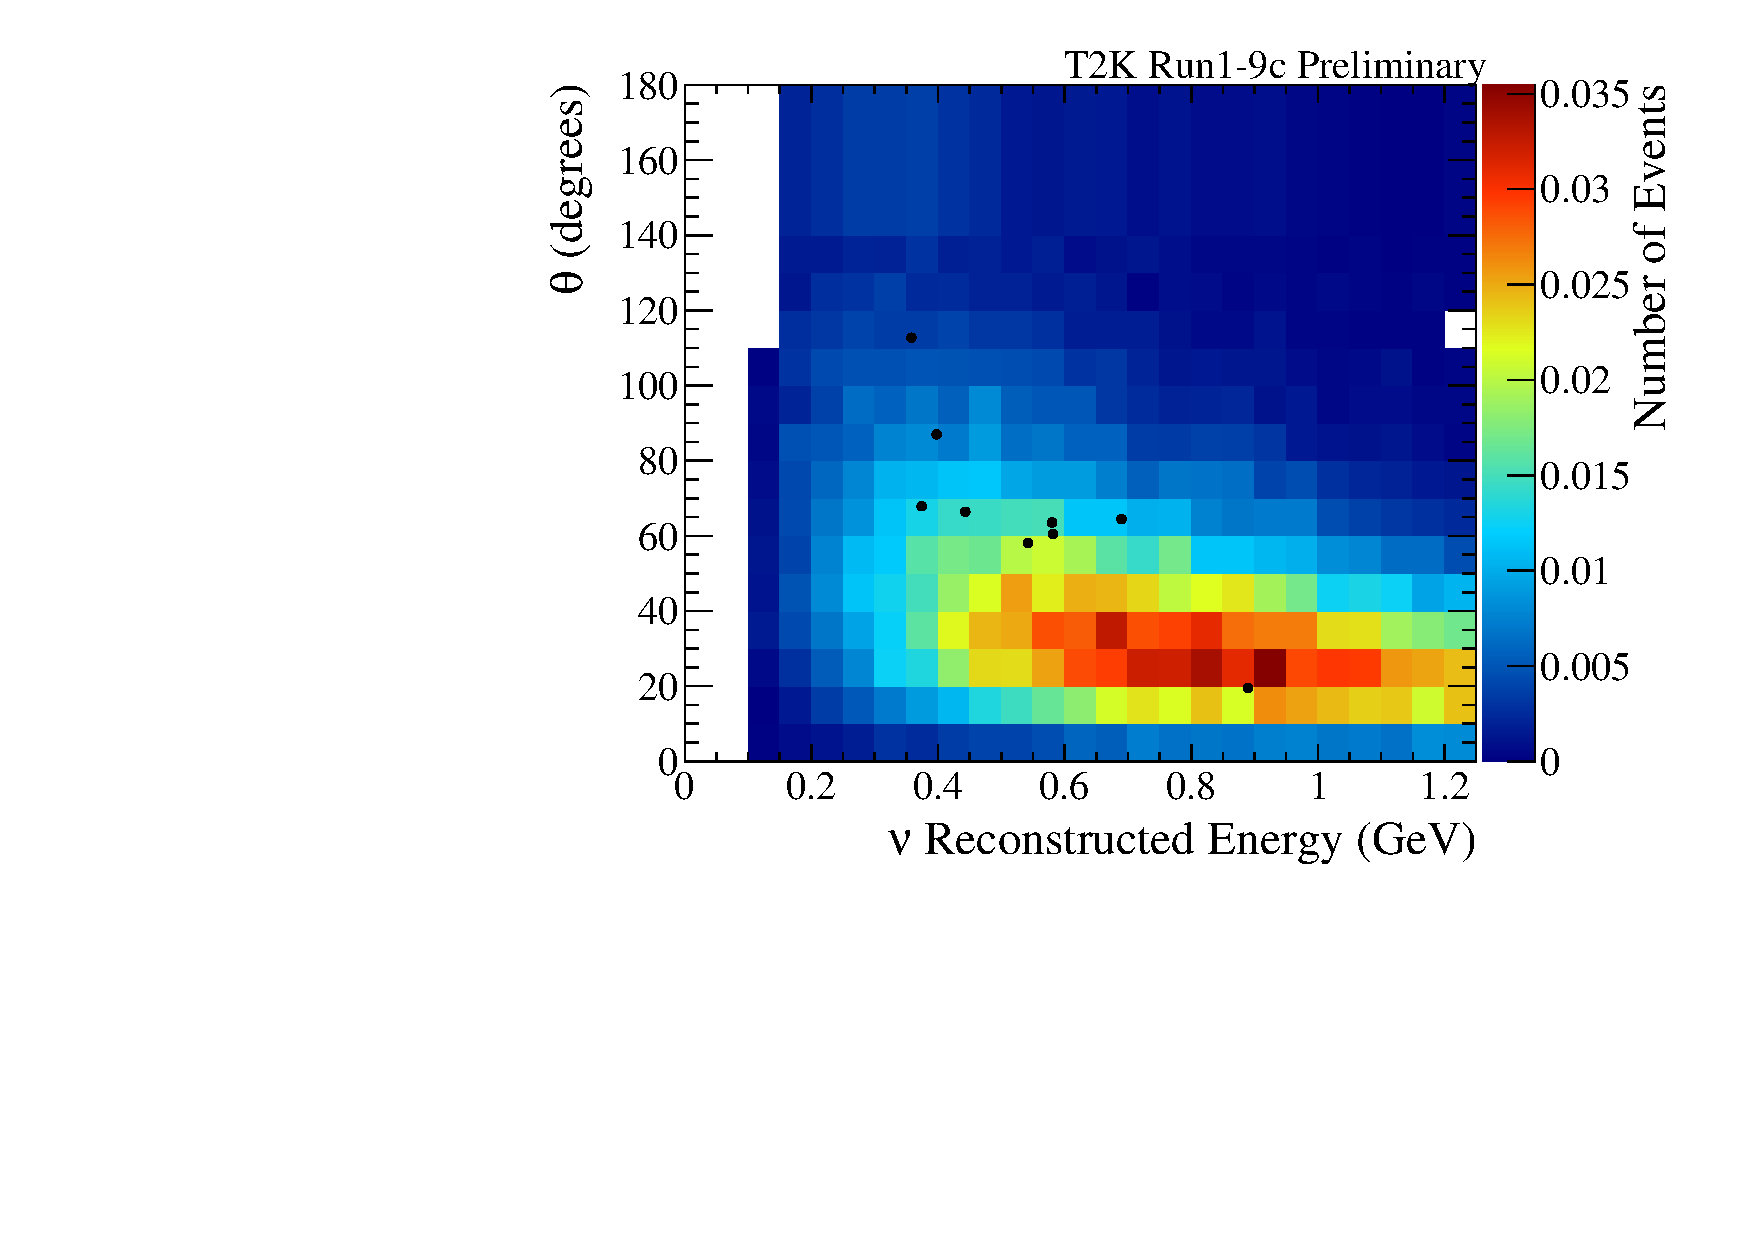
\includegraphics[width=0.9\textwidth]{spectra/components/spectrum_AsmovA_RHC1Re_NueBeam}
		\caption{Intrinsic $\nue$ + Intrinsic $\nueb$}
	\end{subfigure}
	\caption {
		Predicted Asimov A Electron-like antineutrino mode spectra broken down by component. The distributions correspond to the statistics collected in the full \RunPeriod data set. The spectra are generated with the oscillation parameters corresponding to the Asimov data set A shown in \cref{tab:osc_params_joint_asimovA}.
	}
	\label{fig:asimova_spectra_components}
\end{figure*}
\clearpage

\FloatBarrier